\section{Fiche de bilan et de syntèse}
\subsection{Présentation de l'activité en entreprise}
\subsubsection{L'entreprise d'accueil}
L’entreprise Kappa Santé a été créée en 2003 par Mr SCHÜCK (médecin de
santé publique) et par Mme TEXIER (pharmacienne) en vue d’apporter des
services de qualité. Avec une expertise ciblée sur les domaines de:
l’épidémiologie, pharmaco- épidémiologie, la constitution d’e-cohortes i et des
interventions en santé publique et numérique, cette société répond aux
demandes à la fois au niveau national et européenne.
Cette CRO (Contract Research Organization) est une SAS (Société Anonyme
Simplifiée) au capital de 50 000 €.
Le siège social de l’entreprise est situé au 4 rue Cléry à Paris, dans le 2e
arrondissement.
Kappa Santé est membre de l’ENCEPP (European Network of Centres for
Pharmacoepidemiology and Pharmacovigilence), de l’AFCROs (association de
CRO) et du pôle compétitivité numérique Cap digital (collectif européen
d’innovateurs).
L’entreprise Kappa Santé est l’entreprise mère de Kap Code depuis 2015. Kap
Code est une entreprise qui récupère des données liées à la santé sur les
réseaux sociaux.
En mars 2023, Kappa Santé a été racheté par Apices, une entreprise CRO
espagnole qui réalise des études cliniques.
À ses débuts, Kappa Santé réalisait des études dans le but de recueillir des
informations sur des médicaments mais depuis 2012, la société s’est diversifiée
et elle est devenue polyvalente en proposant des services comme le suivi et le
monitoring, la création de protocole, ...
De grosses entreprises comme Pfizer, Janssen, AstraZeneca, Microsoft, IBM... font confiance à Kappa Santé. Les principaux concurrents de Kappa Santé sont
Aixial, Axonal, Cemka, Clinact, Euraxi, Icon, Icta, Iqvia, Sanoïa...

L’équipe dont je fais partie intègre le Département Informatique où M. BRUNAT est le directeur informatique.
Nous développons en Java à l’aide du Framework JSF (Java Server Faces) et
des composants PrimeFaces.
\begin{figure}[H]
    \centering
    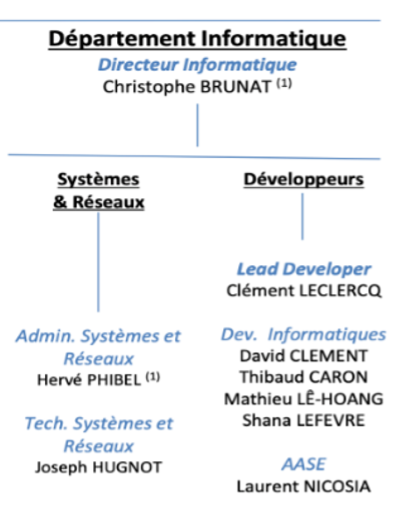
\includegraphics[width=0.4\textwidth]{fiche_bilan/fiche_bilan_images/organigramme_info.png} 
    \caption{Organigramme de l'entreprise}
\end{figure}
Pour communiquer avec notre base de données (développeur), JPA définit des
entités qui sont une instance de classe et nous permet d’écrire des
programmes qui interagissent avec la base de données.
\begin{figure}[H]
    \centering
    \includegraphics[width=0.3\textwidth]{fiche_bilan/fiche_bilan_images/intégration_jpa.png} 
    \caption{Schéma d'intégration de JPA}
\end{figure}

\subsubsection{Le maître d'apprentissage}
Notre équipe est composée de cinq développeurs dont un « lead developer »,
Monsieur Clément LECLERCQ (voir schéma précédent). C’est notre superviseur et il
également mon maître d’apprentissage. Il développe également sur les projets.
Notre objectif est d’assurer le développement et la maintenance de tous nos outils informatisés de recueil de données en utilisant des langages et des outils
de développement.
\subsubsection{Résumé des travaux proposés par l'entreprise}
L'intitulé de mon contrat d'apprentissage est « Développeur Java ».
Mon activité principale est de développer et d’entretenir des applications
\(electronic Case Report Forms\). Ces formulaires permettent de collecter des données cliniques de manière structurée et sécurisée. Ils sont utilisés dans le cadre d'études cliniques pour recueillir des informations sur les patients, les traitements administrés, et les résultats obtenus. Mon rôle consiste à développer ces e-CRF en respectant les spécifications fournies par les chefs de projet et les Data Managers, tout en assurant leur bon fonctionnement et leur conformité aux exigences réglementaires.\
Pour développer des études, nous partons d'une application dites "starter" qui
permet de créer un e-CRF. Cette application est une sorte de modèle qui nous
permet de créer un e-CRF. Nous la faisons évoluer en fonction des
besoins de l'étude. Les dead-line varient en fonction de la taille de l'étude et de la
complexité de l'e-CRF. 
\subsubsection{Travaux effectués en entreprise}
Mon activité au sein de l’entreprise est de développer et d’entretenir des
applications, des
formulaires en ligne nommés de e-CRF.
Tout au long de l’année, j’ai poursuivi mon apprentissage dans le
développement en utilisant les Bonnes Pratiques de développement de Kappa
Santé.
Pour mener à bien notre projet, nous travaillons avec un chef de projet ainsi
qu’avec un Data Manager.
Cette année, j’ai épaulé mes collègues sur leurs projets en développant
diverses fonctionnalités :
\begin{itemize}
    \item Création d’envoi mails automatiques aux utilisateurs : automatiser l’envoi
    de mails en fonction des évènements qui se passent sur l’application, par
    exemple, l’insertion d’un
    patient par un utilisateur, un récapitulatif quotidien des évènements
    indésirables...
    \item Résolution de bugs, à la suite d’une demande sur notre logiciel Redmine,
    \item Réalisation des Phases Listener : C’est un outil propre à JSF (Java Server
    Faces). C’est une interface implémentée par des objets notifiés sur le début
    ou la fin d’un traitement,
    d’un cycle. Ainsi, nous pouvons personnaliser le comportement de nos e-
    CRF. La principale utilisation des Phase Listener est de vider les sous-
    champs entre les pages. On s’en sert pour vider les sous-champs entre les
    pages.
    \item Implémentation des contrôles bloquants et non-bloquants : Ce sont des
    contrôles qui permettent de savoir si la donnée correspond aux attentes du
    e-CRF. Un contrôle bloquant nécessite que l’utilisateur corrige la donnée non-conforme avant
    de pouvoir passer à la page suivante du questionnaire. En revanche, pour
    un contrôle non-bloquant, un message avertit simplement l’utilisateur de la
    non-conformité avant qu’il ne puisse continuer. Tous ces contrôles sont spécifiés dans le document « Data Validation Plan », qui contient toutes les
    instructions nécessaires à la réalisation des contrôles.
    \item Implémentation des Locked Queries : C’est une fonctionnalité propre à
    Kappa Santé. Ils permettent de bloquer, verrouiller, griser, et rendre
    inaccessible un champ enfant
    lorsque la case parent est cochée. Cette fonctionnalité est précieuse car
    elle évite l’enregistrement de données inutiles dans la base de données.
    Ainsi, l’utilisateur ne peut
    pas entrer des informations dans les champs. Pour faire ces modifications,
    j’utilise le fichier xhtml associé au formulaire avec une condition d’affichage
    « rendered ».
\end{itemize}


Mes missions sont également :
Création de fiches de procédures, la participations aux réunions. 
Aujourd’hui après quelques mois au sein de l’entreprise, j’ai mes propres
études. Tout commence par la création de l’étude avec la mise en place tout ce
dont nous avons besoin pour son bon déroulement (base de données…). Au
cours du développement de l’étude, on retrouvera les fonctionnalités vue
précédemment.

%\subsection{Présentation et synthese du sujet de mémoire de l'apprenti}
%\subsubsection{Présentation du sujet de mémoire sur lesquels les apports sont novateurs}
%\subsubsection{Ce qui est déjà connu sur le sujet traités dans le mémoire}
%\subsubsection{Ce que mon travail de mémoire apporte de nouveau}
%\subsubsection{Utilisation potentielle des travaux de votre sujet de mémoire}
%\subsubsection{Principales perspectives des travaux}
